%------------------------------------------------------------
%------------------------------------------------------------
\section{Introduction}
\label{sec:introduction}

Course organization %in universities
involves strategic, tactical and operational decisions relating to curriculum design, student sectioning, course staffing, room planning, 
%equipment provisioning, 
class scheduling and resource allocation \cite{overview_uctp_2016_malaysian}.
The scope %and dynamics 
of these problems and the coordination of the different stages
vary between higher-education systems and institutions 
as does the level of process automation and decision tool support.
In french universities for instance, curricula are conventionally revisited every 5 years and 
students enroll in courses prior to each teaching period in the course of the academic year. %and are partitioned into groups based on their demand profile. 
Demand is matched by sectioning courses into classes, partitioning students %with identical profiles 
into fixed groups, and populating classes with groups. %to match demand.
Eligible groups, %faculty 
teachers, rooms and equipment are then identified for each course before class sessions get scheduled and allocated the necessary resources (see Figure~\ref{fig:utp-workflow}). 
Each stage involves 
different stakeholders with their own requirements
(faculty departments, administrative units, course owners, lecturers, etc.) 
and the workflow naturally allows for deviations and contingencies (marginal amendments to curricula on a yearly basis, late student registrations, staff absences, etc.).

% For one-column wide figures use
\begin{figure}[h]
\begin{center}
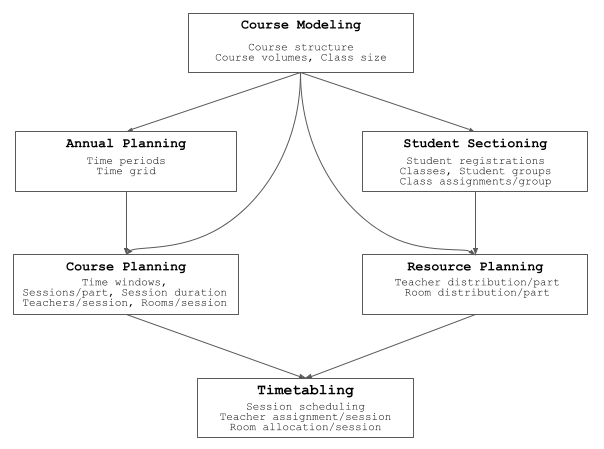
\includegraphics[width=\columnwidth]{img/utp_workflow.png}
\end{center}
\caption{Conventional workflow for course organization in french universities}%: steps and roles}

\label{fig:utp-workflow}
\end{figure}

We introduce in this paper a domain-specific language modeling a broad class of university timetabling problems ({\UTP}) that reduce to hard constraint satisfaction problems ({\CSP}). 
The {\UTP} language allows to mix and match features relating to course scheduling, resource allocation and student sectioning in order to tailor problem instances to each particular environment.
It is designed around a formal domain model and a predicate language to state rules and constraints. 
Each instance is decomposed into a model of entities and maps, a rule set and a solution component. 
Rules express collections of timetabling constraints %that represent 
%assignment decisions %, domain restrictions 
%and general 
%timetabling constraints 
on model entities and 
the solution component %is a list of choices made for some or all of the decisions at stake % (e.g., start time of a session) 
lists assignment decisions. 
The latter does not have to be exhaustive (e.g., it may be void), nor consistent. 
{\UTP} instances may therefore be used to model subproblems and solution seeds %when the whole problem is solved in successive stages (e.g., sequential workflows chaining student sectioning, course scheduling and resource allocation). 
%Since no assumption is made on the computing task, 
%{\UTP} instances may also be used
either to repair timetables, complete partial timetables or generate full solutions. 

%Similarly to the schema proposed in \cite{2018muller,ITC2019} for the international timetabling competition ({\ITC}), 
The {\UTP} model adopts:
\begin{itemize}
    \item a multi-scale schedule horizon, i.e., weeks, weekdays and daily slots ;
    \item a mixed set of resources, i.e., students, rooms and teachers ;
    \item a hierarchical course structure, i.e., a course (e.g. algorithmic) contains course parts (e.g., algorithmic practice), a course part contains classes (e.g., algorithmic practice for student group G1a), and a class contains sessions (e.g., the third session of algorithmic practice for G1a).
\end{itemize}
In our approach, class sessions are considered as first-class objects that must be scheduled individually alongside resources. %For full flexibility, 
%\todo[inline]{"part classes" on n'utilise plus ce terme après, mais "class", donc je trouve que c'est piégeux, parce que ce dont on parle ici "part classes" est appelé plus tard "class". Je sais que l'intro est déjà longue, mais je m'interroge quand même sur l'intérêt de ne pas donner plus de détails (à la place de "i.e. course parts...") du type "i.e. a course (e.g. algorithmic) contains course parts (e.g. algorithmic lectures), a course part contains classes (e.g. algorithmic lectures for student group G1a), and a class contains sessions (e.g. the third session of algorithmic lecture for G1a)". C'est à mon avis très important que lecteur comprenne les termes dès le début de l'intro. }
%\marc{On n'utilise jamais "course parts", "part classes" et "class sessions" mais "part", "classes" et "sessions", ici je ne trouve pas ça gênant d'insister sur le lien puisqu'on parle de la hiérarchie ?}
%\todo[inline]{DL : Il faut savoir que ce n'est pas le cas dans ITC, est-ce que le lecteur "visé" le sait ? Ca ne vaudrait pas le coup d'en dire un mot ?}
%\marc{En relisant c'est bien indiqué "in our approach however" donc ça indique bien que ce n'est pas le cas pour ITC ?}
The scheduling scheme assumes cumulative resources and multi-resource sessions 
but may be adapted to each instance using entity properties and maps. 
Specifically, 
sessions are cast as single-resource %tasks 
(e.g., face-to-face lectures) or multi-resource tasks (e.g., hybrid sessions) %using multiplicity marking 
by quantifying the needed resources. 
%In either case, 
Candidate resources for a session are identified based on the distribution that is given over courses (i.e., registered students) and course parts (i.e., designated teachers and rooms). 
The volumes of sessions are themselves configurable for teachers (i.e., sessions quota per course part) but pre-determined for students (i.e., mandatory session attendance per class) while rooms may be reused at will. %within course part boundaries. 

No limits apply on simultaneous resource usage but for rooms whose hosting capacity must match %cumulated 
class size. 
As for session scheduling, start time grids are configurable in each course part and 
the model simply requires full session sequencing in each class. 
Any resource may therefore be assigned simultaneous or overlapping sessions  (e.g., joint sessions, optional tutoring) except for rooms assigned to a multi-room session. 
Note that disjunctive rules may be enforced as needed to prevent parallelism or impose unit resources. 
%are subject to class-scoped global sequencing constraints 
%
%Lastly, the model sections students into classes (each part of a requested course is mandatory) and supports subgroup inclusion constraints between classes. 
Lastly, the model partitions students into groups and assign groups to classes consistently with predefined class capacities and any subgroup inclusion constraint expressed between classes.
%TODO last sentence on groups: 
Note that student groups are considered a by-product of student sectioning and as such may only be listed in the solution component. 

%Rules denote conjunctions of {\UTP} constraints that are formed by instantiating built-in predicates. %on sessions of entities. 
The predicate language allows to state additional constraints %on sessions and entities 
on a common type of objects called e-maps 
that represent conditional assignments of sessions to entities. 
Formally, {\UTP} constraints apply to one or more e-maps and may involve parameters
based on predicate signatures. 
%are {\CP} abstractions representing %denoting  
%assignment decisions (e.g., allocation of a room to a session)
%domain restrictions (e.g., teacher unavailability), 
%or general timetabling constraints (e.g., session sequencing). 
%A {\UTP} constraint applies to one or more objects called e-sessions and possible parameters based on the predicate's signature. 
%{\UTP} constraints apply to the same type of objects, called e-maps, and possibly parameters based on predicate signatures. 
Each e-map associates an entity to a subset of its compatible or constitutive sessions 
%(resource or course element) 
%An e-map is either a resource mapped to some or all of its candidate sessions, a course element mapped to some or all of its constitutive sessions, or a self-mapped session. 
and %serve to restrict the scope of constraints and 
is interpreted as 
%prescriptive %session-to-entity assignments when they appear in assignment constraints, 
a set of conditional %session-to-entity 
assignments, % within constraints, % otherwise,  %by {\UTP} constraints 
%(except for the particular case of assignment constraints). 
%unconditional session assignments in the particular case of {\UTP} assignment constraints, 
%or as conditional assignments otherwise.  
%Specifically, %(non-assignment) 
%the scope of the 
that is, 
a constraint is %conditionally restricted to 
only 
evaluated on the sessions whose committed assignments match its e-map argument(s). 
%For instance, a time restriction constraint on a resource s-domain will only be effective on the sessions in that domain which are assigned to that resource. 
%Each predicate may be applied indistinctly to resources or course elements . 
%Predicates indistinctly apply to resources or course elements (e.g., start time restrictions) and serve to constrain the possible sessions of resources (e.g., unavailabilities of a teacher) or the constitutive sessions of course elements (e.g., periodicity of a class). 
E-maps may then be adjusted 
to constrain candidate sessions of resources (e.g., teacher unavailability), 
constitutive sessions of course elements (e.g., class periodicity), 
or individual sessions (e.g., session sequencing and parallelization).
Note that each predicate may be applied indistinctly to sessions of resources or course elements. 
Besides, constraints on e-maps modeling constitutive sessions are de facto 
unconditional. 

Rules are used to state individual constraints as well as 
collections of constraints 
on selected classes of entities and sessions 
(e.g., disjunctive scheduling rules for teachers, time restrictions on the courses of a curriculum). 
Each rule is tied to a predicate and 
defined by a universally quantified %constraints build with timetabling 
%atomic
formula wherein bounded quantifiers restrict the domain of each e-map variable. % of the chosen predicate. 
%The rule language provides a comprehension syntax based on entity selectors and domain filters %on entities and sessions to denote bounded quantification. 
A formal syntax of selectors is provided to build and filter domains of e-maps 
based on session ranks% within classes
, entity identifiers and types, or any user-defined class of elements (e.g., team of lecturers, block of rooms). 
A rule hence denotes the conjunction of constraints obtained by instantiating its predicate over the cross-product of the domains of its e-map variables. 

The language is implemented as an external {\DSL} using {\XML}. %and {\JSON} \cite{} formats 
%and is also embedded in two constraint modeling languages, namely, {\MINIZINC} \cite{MZN} and {\CHR} \cite{CHR}. 
%\marc{Finalement on ne présente pas CHR mais on en parle juste en conclusion.}
%Specifically, w
The implementation includes 
%The {\UTP} language is solver as an external {\DSL} in the form of an {\XML}  language. 
%As for implementation, 
an {\XML} schema to encode rule-based {\UTP} instances 
and a tool chain %to convert and solve instances using alternative constraint languages, namely, {\MINIZINC} \cite{MZN} and {\CHR} \cite{CHR}. 
consisting of
an {\XML} parser, 
a rule processor to flatten rules into constraints, 
and a {\JSON} encoder to convert the constraint-based instances to solver-compatible formats.
%using {\JSON} and {\DZN} ({\MINIZINC} input data format). 
%to rewrite model and solution components using specific domain and assignment predicates,  
%and the alternative constraint-based models in {\MINIZINC} and {\CHR}.
%Beyond {\MINIZINC} and {\CHR},
{\JSON}-encoded instances may be used as inputs to any solver 
implementing the model, solution scheme, and predicates of the {\UTP} language.
%We present here a generic constraint programming ({\CP}) model and discuss its implementation in {\MINIZINC} and {\CHR}.
As an early proof of concept, we report experiments on timetabling instances modeling undergraduate curricula in a French university and solved with \CP{} solvers. 
The detailed {\XML} specification of the language and the instance formats  
are beyond the scope of this paper and may be found at \cite{USPsite} 
which also provides %access to
the \CP{} models we developed, 
the tool suite, and
a benchmark of instances.

The remainder of the paper is organized as follows.
Section~\ref{sec:schema} introduces the {\UTP} language and its semantics.
Section~\ref{sec:related-work} compares the \UTP{} language with the schema proposed in \cite{2018muller,ITC2019} for the international timetabling competition ({\ITC}).
Section~\ref{sec:model_implementation} presents the {\CP} model for the {\UTP} class and the experiments we performed.
%Section~\ref{sec:experimentations} illustrates the applicability of the language on a real case study. %with {\Minizinc} and {\CHR}.
Section~\ref{sec:conclusion} concludes and discusses extensions of this work.